\documentclass{article}
\usepackage[utf8]{inputenc}
\documentclass[12pt]{article}
%\usepackage[left=3cm, right=2.5cm, top=2.5cm, bottom=2.5cm]{geometry}e}
\usepackage[utf8]{inputenc}
\usepackage[spanish,english]{babel}
\usepackage{apacite}
\usepackage[round]{natbib}
\usepackage{hyperref}
\usepackage{float}
\usepackage{svg}
\usepackage[margin = 1in, top=2cm]{geometry}% Margins
\setlength{\parindent}{2em}
\setlength{\parskip}{0.2em}
\usepackage{setspace} % Setting the spacing between lines
\usepackage{amsthm, amsmath, amsfonts, mathtools, amssymb, bm} % Math packages 
\usepackage{svg}
\usepackage{graphicx}
\usepackage{pgfplots}
\usepackage{epstopdf}
\usepackage{subfig} % Manipulation and reference of small or sub figures and tables
\usepackage{hyperref} % To create hyperlinks within the document
\spacing{1.15}
\usepackage{appendix}
\usepackage{xcolor}
\usepackage{cancel}
\usepackage{enumerate}
\usepackage[shortlabels]{enumitem}


\usepackage[round]{natbib}
%\bibliographystyle{plainnat}
\bibliographystyle{apacite}


\newtheorem{defin}{Definition.}
\newtheorem{teo}{Theorem. }
\newtheorem{lema}{Lemma. }
\newtheorem{coro}{Corolary. }
\newtheorem{prop}{Proposition. }
\theoremstyle{definition}
\newtheorem{examp}{Example. }
\newtheorem{problem}{Problem}
\newtheorem{subproblem}{}[problem]
% \numberwithin{problem}{subsection} 

\newcommand{\card}{\operatorname{card}}
\newcommand{\qiq}{\qquad \implies \qquad}
\newcommand{\qiffq}{\qquad \iff \qquad}
\newcommand{\qaq}{\qquad \textbf{and} \qquad}
\newcommand{\qoq}{\qquad \textbf{or} \qquad}
\newcommand{\settf}{\text{ \emph{:} }}
\newcommand{\chbox}{\makebox[0pt][l]{$\square$}\raisebox{.15ex}{\hspace{.9em}}}
\newcommand{\cchbox}{\makebox[0pt][l]{$\square$}\raisebox{.15ex}{\hspace{0.1em}$\checkmark$}}

\title{Problem Set 1}
\author{Mitchell Valdés-Bobes}
\date{November 12, 2020}

\begin{document}

\maketitle

\subsection*{Problem 1}

\subsubsection*{(a)}

Consider the state variables $A$ the assets holdings in the current period and $\tilde{c}$, last period consumption and the decision variables $c$ current period consumption and  $A'$ the assets that will be carried to the next period. The the \textbf{Bellman Equation} is:

$$\left.V(A, x)=\max _{(c, A^{\prime}) \in \Gamma(A,\tilde{c})} \left\{ u\left(c, \tilde{c}\right)+\beta V\left(A^{\prime}, c\right)\right \}$$

the feasible correspondence is:

$$\Gamma(A,\tilde{c}) = \Gamma(A) = \{(c, A')\in \mathbb{R}^2|A'\geq 0, c\geq 0, A' = R(A-c)\}

We can reduce the problem to:

$$\left.V(A, \tilde{c})=\max _{A^{\prime} \in \Gamma(A)} \left\{ u\left(A-\frac{A^{\prime}}{R}, \tilde{c}\right)+\beta V\left(A^{\prime}, A-\frac{A^{\prime}}{R}\right)\right \}$$

If we assume $(\Gamma 1)$, $(\Gamma 2)$, $(\Gamma 3)$, $(F1)$, $(F2)$, $(F3)$ and $(F4)$ from class; then the solution of the \textbf{Bellman Equation} is unique, with a strictly increasing, strictly concave value function that is differentiable on the interior of the feasible set.

The conditions for optimally are:

\begin{align*}
    \text{FOC:}&\qquad 0 = -u_{c}\left(A-\frac{A^{\prime}}{R}, \tilde{c}\right) + \beta\left[V_{A'}\left(A^{\prime}, A-\frac{A^{\prime}}{R}\right) -\frac{1}{R}V_{\tilde{c}}\left(A^{\prime}, A-\frac{A^{\prime}}{R}\right) \right] \\
    \text{Env:}& \qquad V_A(A,\tilde{c}) = u_c(c,\tilde{c})\frac{\partial c}{\partial A} \qaq V_A(A, \tilde{c}) = u_\tilde{c}(c,\tilde{c})
\end{align*}

Combining the above:

$$u_{c}\left(A-\frac{A^{\prime}}{R}, \tilde{c}\right) = \beta\left[u_c(c,\tilde{c}) - \frac{1}{R}u_{\tilde{c}}(c,\tilde{c})  \right]$$

\subsubsection*{(b)}
We can re write the problem 
$$\max_{c_t}\sum_{t=0}^{\infty}{\beta^t(\ln c_t + \gamma \ln c_{t+1})}$$ as

$$\max_{c_t}\sum_{t=0}^{\infty}{\beta^t\ln c_t} + \gamma \sum_{t=0}^{\infty}{\beta^t+1 \ln c_{t+1}} + \gamma \ln c_{-1}$$

which reduces to:
$$\max_{c_t} [1+\beta\gamma] \sum_{t=0}^{\infty} \beta^t\ln c_t }$$

\subsubsection*{(c)}

\subsection*{Problem 2}
\subsubsection*{(a)}
The sequence problem is
$$
\begin{array}{r}
\max _{\left\{x_{t+1}\right\}_{t=0}^{\infty}} \sum_{t=0}^{\infty} \delta^{t}\left(a x_{t}-\frac{1}{2} b x_{t}^{2}-\frac{1}{2} c\left(x_{t+1}-x_{t}\right)^{2}\right) \\
\text { s.t. } \quad 0 \leq x_{t+1} \leq x_{t}
\end{array}
$$
The Bellman equation is
$$
V\left(x_{t}\right)=\max _{x_{t+1}} \quad a x_{t}-\frac{1}{2} b x_{t}^{2}-\frac{1}{2} c\left(x_{t+1}-x_{t}\right)^{2}+\delta V\left(x_{t+1}\right)\right
$$
Considering: 
$$
F(x, y)=a x-\frac{1}{2} b x^{2}-\frac{1}{2} c(y-x)^{2}
$$
The $T$ operator is
$$
T v(x)=\max _{y} \left\{ F(x,y) +\delta v(y)\right\}
$$
\subsubsection*{(b)}
We can make $y=x$ every period, if $y<x$ we will get less profits. This implies $F(x,x) = a x-\frac{1}{2} b x^{2}$ with FOC:
$$x^*=\frac{a}{b}$$. 

Substituting 
$$
F\left(x^*, x^* \right)=\frac{1}{2} \frac{a^{2}}{b}
$$

Going back to  sequential problem
$$
\begin{aligned}
V\left(x_{0}\right) &=\max _{\left\{x_{i+1}\right\}_{t=0}^{\infty}} \sum_{t=0}^{\infty} \delta^{t}\left(a x_{t}-\frac{1}{2} b x_{t}^{2}-\frac{1}{2} c\left(x_{t+1}-x_{t}\right)^{2}\right)
& \leq \frac{1}{2} \frac{a^{2}}{b} \frac{1}{1-\delta}=\widehat{v}
\end{aligned}
$$
\subsubsection*{(c)}
$$
\begin{aligned}
T \hat{v}(x) &=\max _{y}\left\{a x-\frac{1}{2} b x^{2}-\frac{1}{2} c(y-x)^{2}+\delta \frac{1}{2} \frac{a^{2}}{b} \frac{1}{1-\delta}\right\}\end{aligned} $$
Using the upper bound:
$$\begin{aligned}
T \hat{v}(x)& \leq \frac{1}{2} \frac{a^{2}}{b}+\delta \frac{1}{2} \frac{a^{2}}{b} \frac{1}{1-\delta} = \frac{1}{2} \frac{a^{2}}{b}\left(1+\frac{\delta}{1-\delta}\right)=\frac{1}{2} \frac{a^{2}}{b} \frac{1}{1-\delta}=\widehat{v}
\end{aligned}
$$


\subsubsection*{(d)} 
Maximizing $y$ and substituting in $T\hat{v}$:
$$
T \hat{v}(x)=a x-\frac{1}{2} b x^{2}+\delta \frac{1}{2} \frac{a^{2}}{b} \frac{1}{1-\delta}
$$
If

$$
\left(T^{n} \widehat{v}\right)(x)=\alpha_{n} x-\frac{1}{2} \beta_{n} x^{2}+\gamma_{n}
$$

Then

$$
\left(T^{n+1} \widehat{v}\right)(x)=\max _{y}\left\{a x-\frac{1}{2} b x^{2}-\frac{1}{2} c(y-x)^{2}+\delta\left(\alpha_{n} y-\frac{1}{2} \beta_{n} y^{2}+\gamma_{n}\right)\right\}
$$

Solving for $y$ we get

$$
y=\frac{c x+\delta \alpha_{n}}{c+\delta \beta_{n}} 
$$

We can obtain:

$$
\begin{aligned}
\alpha_{n+1} &=a+\frac{\alpha_{n}}{c+\delta \beta_{n}} c \delta,
\beta_{n+1} &=b+\frac{\beta_{n}}{c+\delta \beta_{n}} c \delta ,
\gamma_{n+1} &=\delta \gamma_{n}+\frac{1}{2} \frac{\alpha_{n}^{2}}{c+\delta \beta_{n}} \delta^{2}
\end{aligned}
$$

(e) Let  $\beta=\lim \beta_{n}, \alpha=\lim \alpha_{n}, \gamma=\lim \gamma_{n},$ 
% $$
% \begin{aligned}
% \beta &=\frac{-(c-\delta(b+c))+\sqrt{(c-\delta(b+c))^{2}+4 b c \delta}}{2 \delta} \\
% \alpha &=a \frac{c+\delta \beta}{c+\delta \beta-\delta c}=a\left(1-\frac{\delta c}{c+\delta \beta-\delta c}\right) \\
% \gamma &=\frac{1}{2(1-\delta)} \frac{\alpha^{2}}{c+\delta \beta} \delta^{2}
% \end{aligned}
% $$
Solve for $\alpha, \beta,$ and $\gamma .$ and check that:

$$
V(x)=\alpha x-\frac{1}{2} \beta x^{2}+\gamma
$$

Then

$$
V(x)=\max _{y}\left\{a x-\frac{1}{2} b x^{2}-\frac{1}{2} c(y-x)^{2}+\delta \alpha y-\frac{1}{2} \delta \beta y^{2}+\gamma \delta\right\}
$$

using the first order condition:

$$
\frac{c x+\delta \alpha}{c+\delta \beta} &=y
$$

$$
\begin{aligned}
& a x-\frac{1}{2} b x^{2}-\frac{1}{2} c\left(\frac{c x+\delta \alpha}{c+\delta \beta}-x\right)^{2}+\delta \alpha \frac{c x+\delta \alpha}{c+\delta \beta}-\frac{1}{2} \delta \beta\left(\frac{c x+\delta \alpha}{c+\delta \beta}\right)^{2}+\gamma \delta 
\end{aligned}
$$
thus:

 $$V(x) = \alpha x-\frac{1}{2} \beta x^{2}+\gamma$$

\subsection*{Problem 3}
\subsubsection*{(a)}
The Bellman equation is:
$$
V(k)=\max _{k^{\prime}, I}\left\{\pi(k)-\gamma(I)+ \left( \frac{1}{R} \right) V\left(k^{\prime}\right)\right\}
$$
substitute $I=k^{\prime}-(1-\delta) k$
$$
V(k)=\max _{k^{\prime}}\left\{\underbrace{\pi(k)-\gamma\left(k^{\prime}-(1-\delta) k\right)}_{F(k,k')} + \frac{1}{R} V\left(k^{\prime}\right)\right\}
$$

The conditions for maximization are:

\begin{align*}
    \text{FOC:}&\qquad \gamma^{\prime}\left(k^{\prime}-(1-\delta) k\right)=\frac{1}{R} V^{\prime}\left(k^{\prime}\right)\\
    \text{Env:}& \qquad V^{\prime}(k)=\pi^{\prime}(k)-(1-\delta) \gamma^{\prime}\left(k^{\prime}-(1-\delta) k\right)
\end{align*}

Combining both conditions we get the \textbf{Euler Equation}:
$$
\gamma^{\prime}\left(k^{\prime}-(1-\delta) k\right)=\frac{1}{R}\left[\pi^{\prime}\left(k^{\prime}\right)-(1-\delta) \gamma^{\prime}\left(k^{\prime \prime}-(1-\delta) k^{\prime}\right)\right]
$$

\subsubsection*{(b)}
If there is a steady state $k=k'=k''=\bar{k}$ then:

\begin{align*}
    \gamma^{\prime}\left(\bar{k}-(1-\delta) \bar{k}\right)&=\frac{1}{R}\left[\pi^{\prime}\left(\bar{k}\right)-(1-\delta) \gamma^{\prime}\left(\bar{k}-(1-\delta) \bar{k}\right)\right]    \\
    &\implies \gamma^{\prime}\left(\delta\bar{k}\right)=\frac{1}{R+1-\delta} \pi^{\prime}\left(\bar{k}\right)
\end{align*}

Then the steady exists if the above equation has a solution and if unique is the solution is unique. If $\gamma$ and $\pi$ are continuous and strictly concave or convex then the steady state will exist.

An increase in $R$ will lead to a decrease in $\bar{k}$ this is because the firm will be less patient thus saving less to favor consumption in the short run.

\subsubsection*{(c)}

$$\gamma^{\prime}\left(I_{i}\right)=I_{i}$$ and $$\pi^{\prime}(k)=-\left(k-k^{*}\right)=k^{*}-k$$

Then we get

$$
I_{l}=\frac{1}{R}\left[k^{*}-k_{t+1}+(1-\delta) I_{t+1}\right]
$$

And substituting $k_{t+1}=(1-\delta) k_{t}+I_{t}$ we have:

$$
I_{t+1}-I_{t}=\left[\frac{R+\delta}{1-\delta}\right] I_{i}+k_{t}-\frac{k^{*}}{1-\delta}
$$

Steady state we need to find $\bar{k}$ that solves $\Delta k=0$ and $\Delta I=0$. Where

The curve 

$$
\Delta I=0 \qiq 
I_{t}=-\left[\frac{1-\delta}{R+\delta}\right] k_{t}+\frac{k^{*}}{R+\delta}
$$

and

$$
\Delta k=0 \qiq I_{t}=\delta k_{t}
$$

\begin{figure}[h]
    \centering
    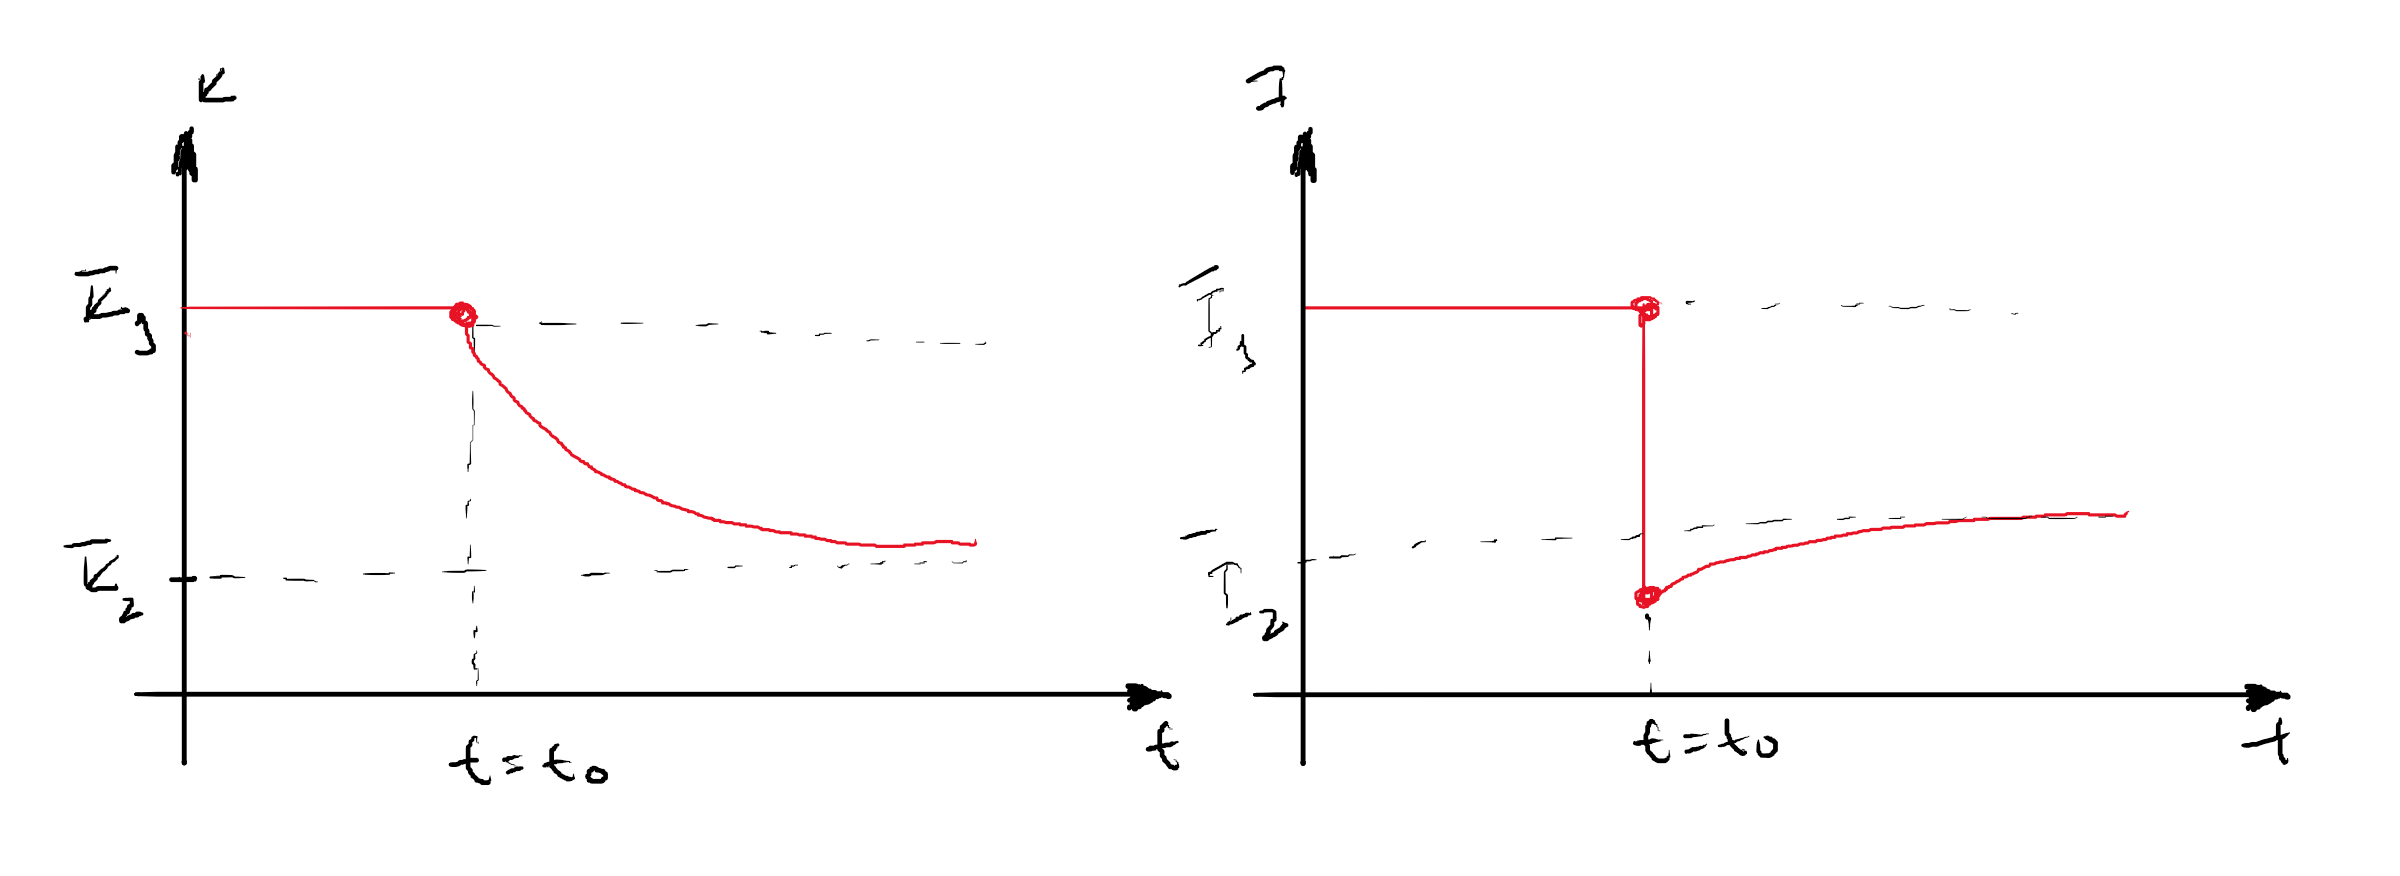
\includegraphics[width=.6\linewidth]{Untitled.png}
    \label{fig:ex2_2}
    \caption{Change in Investment and Capital}
\end{figure}



\subsection*{Problem 4}
\subsubsection*{(a)}
Let
$$u(c,G) = \frac{\left(c G^{\eta}\right)^{1-\gamma}}{1-\gamma}$$

and

$$k'=(1-\delta) k+f\left(k\right)-c$$

The \textbf{Bellman Equation is:}

$$V(k,G) = \max_{k'}\left{\{u(c,G)-\beta V(k', G)\right\}$$

The conditions for maximization are:
\begin{align*}
\text{FOC:}& \quad -u'((1-\delta)k+f(k)-k',G)+\beta V'(k',G')\\
\text{Env:}& \quad V'(K, G)=u'\left(f(k)+(1-\delta) k-k', G\right)\left[f'(k)+1-\delta\right]\\
\end{align*}

Considering that $$k'=g(k) \qquad k''=g(g(k))$$ being $g(\cdot)$ the optimal investment policy then combining \textbf{FOC} and \textbf{Env} we get:
$$u'((1-\delta)k+f(k)-k',G) = \beta u'\left(f(k')+(1-\delta) k'-k'', G'\right)\left[f'(k')+1-\delta\right]$$

Going back to the sequential formulation and using the specific functional form we get the difference equations governing the
evolution of consumption and capital along an optimal path:

$$\left\{
\begin{array}{cc}
    \left(\frac{c_t}{c_{t+1}}\right)^\gamma = \beta \left(\frac{G_{t+1}}{c_{t}}\right)^\eta(1- \gamma) (1-\delta f'(k_{t+1}))   \\
    k_{t+1}=(1-\delta) k_t+f\left(k_t\right)-c_t
\end{array}
$$

\subsubsection*{(b)} 
Using the previous results, and $G_{t+1} = g G_t$ and setting $c_t=\bar{c}$, $k_t=\bar{k} $ for all $t$, Euler equation becomes 
$$\frac{g^{\eta(\gamma -1 ) }}{\beta}-1+\delta = f'(\bar{k})$$
Notice that the left hand side ($\frac{g^{\eta(\gamma -1 ) }}{\beta}>1$ since $g>0$, $\beta<1$ and ${\eta(\gamma -1 )>0 $ ) and the right hand side (by $f$ increasing) are positive, and the INADA conditions guarantee the existence of a  unique steady state solution for $\bar{k}$.

Consumption follows from the budget constraint:
$$ \bar{c}=f(\bar{k}) -\delta \bar{k}$$
\subsubsection*{(c)} Long run dynamics: \begin{itemize}
    \item As $g$ increases, $f'(k)$ increases, which by concavity of $f$ implies $\bar{k}$ decreases. 
    \item Since steady state $k$ drops, $c$ drops as well. This is explained by the following equation and the SS equation of capital:
    $$\frac{\partial \Bar{c}}{\partial \bar{k}}= f'(k)-\delta>0$$
\end{itemize}
In conclusion, both capital and consumption decrease in the long run.

In the short run, we expect a sudden increase in consumption after the shock at $t_o$, since the allocation of capital  for  the next period will be smaller. Capital will decrease gradually until reaching the new SS.
 \end{document}